% supplement.tex -- included at the end of main.tex
\clearpage
\renewcommand{\thefigure}{S.\arabic{figure}}
\renewcommand{\thetable}{S.\arabic{table}}
\renewcommand{\theequation}{S.\arabic{equation}}
\setcounter{figure}{0}
\setcounter{table}{0}
\setcounter{equation}{0}

 {\LARGE \noindent \textbf{Supplementary Material}}

%=====================================================================
\subsection*{S1. Hydrodynamics}

\paragraph{S1.1 Navier--Stokes equations.} Mass conservation in a material volume $V(t)$ gives $\frac{d}{dt}\int_V\rho\,dV=0$. The Reynolds transport theorem turns this into the continuity equation
\begin{equation}
\frac{\partial\rho}{\partial t}+\nabla\cdot(\rho\bm u)=0 ,
\end{equation}
which reduces to $\nabla\cdot\bm u=0$ for an incompressible fluid. Momentum balance on the same volume, with surface stresses $\bm\sigma\cdot\hat{\bm n}$ and body force $\bm f$, gives Cauchy's equation
\begin{equation}
\rho\frac{D\bm u}{Dt}=\nabla\cdot\bm\sigma+\bm f .
\end{equation}
For a Newtonian fluid, $\bm\sigma=-p\bm I+\eta\left(\nabla\bm u+\nabla\bm u^{T}\right)$. With $\nabla\cdot\bm u=0$ this yields the incompressible Navier--Stokes equations.

Lengths are scaled by $a$, velocities by $U$ and pressure by $\eta U/a$. Then
\begin{equation}
\mathrm{Re}\left(\frac{\partial\bm u}{\partial t}+\bm u\cdot\nabla\bm u\right)=-\nabla p+\nabla^2\bm u+\bm f,\qquad \mathrm{Re}=\frac{\rho Ua}{\eta}.
\end{equation}
For \textit{E.~coli} ($a\approx1\,\mu$m, $U\approx30\,\mu$m\,s$^{-1}$, water), $\mathrm{Re}\approx3\times10^{-5}$. For a phage the value is smaller still. The inertial terms are therefore dropped, which gives the Stokes equations\cite{purcell1977life,happel1983}.

\paragraph{S1.2 Stokes flow past a translating sphere.} The sphere has radius $R$ and velocity $\bm v$, and the fluid is at rest at infinity. Linearity and isotropy restrict the solution to the form
\begin{equation}
\bm u(\bm r)=A(r)\,\bm v+B(r)\,\frac{\bm r(\bm v\cdot\bm r)}{r^2}.
\end{equation}
The general solution is a combination of a Stokeslet (decaying as $1/r$) and a source dipole (decaying as $1/r^3$),
\begin{equation}
\bm u=A_1\left(\frac{\bm v}{r}+\frac{\bm r(\bm v\cdot\bm r)}{r^3}\right)+A_2\left(\frac{\bm v}{r^3}-\frac{3\bm r(\bm v\cdot\bm r)}{r^5}\right).
\end{equation}
No slip, $\bm u(|\bm r|=R)=\bm v$ for every direction $\hat{\bm r}$, gives two conditions:
\begin{equation}
\frac{A_1}{R}+\frac{A_2}{R^3}=1,\qquad \frac{A_1}{R}-\frac{3A_2}{R^3}=0
\quad\Longrightarrow\quad A_1=\frac{3R}{4},\quad A_2=\frac{R^3}{4}.
\end{equation}
Substitution recovers Eq.~\eqref{eq:stokes_sphere}. The drag follows from the Stokeslet strength, $\bm F=-8\pi\eta A_1\bm v=-6\pi\eta R\bm v$. This is the drag used for the phage friction coefficient $\gamma=6\pi\eta R_P$.

\paragraph{S1.3 Rotating sphere and the inertial correction (remark).} A sphere rotating at $\bm\omega$ generates the rotlet flow $\bm u_0=R^3\bm\omega\times\bm r/r^3$. The disturbance pressure is identically zero. One of the source notes adds the first inertial correction, a secondary flow $\bm u_1$ that draws fluid in at the poles and pushes it out at the equator. This $\bm u_1$ was proposed as a ``non-laminar vortex'' that could attract phage toward the cell.

\note{This correction scales as $\mathrm{Re}_\omega=\rho\omega R^2/\eta$ relative to $\bm u_0$. For the cell body, $\omega\sim 10$--$20$\,rad\,s$^{-1}$ and $R\sim1\,\mu$m give $\mathrm{Re}_\omega\sim10^{-5}$. For the flagellar bundle ($\omega\sim 600$\,rad\,s$^{-1}$, $R\sim 10$\,nm) it is smaller still. The secondary flow cannot produce a measurable attraction, so it is omitted from the model. The point is kept here because it appears in earlier drafts.}

%=====================================================================
\subsection*{S2. Phage--receptor first-passage times}
Consider independent particles in a deep potential well $U(x)$. They are initially inside the well and slowly leak out across the barrier. The overdamped Langevin equation $\gamma\dot x=-U'(x)+\eta(t)$ produces probability densities $P(x,t)$ that obey the Fokker--Planck (Smoluchowski) equation
\begin{equation}
\frac{\partial P}{\partial t}=\frac{\partial}{\partial x}\left(\frac{U'}{\gamma}P\right)+D\frac{\partial^2P}{\partial x^2}
= D\frac{\partial}{\partial x}\left[e^{-\tilde U}\frac{\partial}{\partial x}\left(e^{\tilde U}P\right)\right],\qquad \tilde U=\frac{U}{k_BT},
\end{equation}
where we used the Stokes--Einstein relation $\gamma D=k_BT$. The initial condition is $P(x,0)=\delta(x-x_0)$. Absorbing boundaries $P(\pm x_A,t)=0$ remove trajectories at their first exit.

\paragraph{Survival and first-passage density.} The survival probability is $S(t)=\int_{-x_A}^{x_A}P\,dx=\mathrm{Prob}(\tau\ge t)$. The first-passage density is then
\begin{equation}
f(t)=-S'(t)=-\int\frac{\partial P}{\partial t}\,dx .
\end{equation}

\paragraph{Characteristic function.} Define $\varphi(\omega)=E[e^{i\omega\tau}]=\int_0^\infty e^{i\omega\tau}f(\tau)\,d\tau$. Integrating by parts in time, with $P\to0$ as $t\to\infty$ and $\int P(x,0)\,dx=1$, gives
\begin{equation}
\varphi(\omega)=1+i\omega\int g(x,\omega)\,dx,\qquad g(x,\omega)=\int_0^\infty e^{i\omega\tau}P(x,\tau)\,d\tau .
\end{equation}
Transforming the Fokker--Planck equation in the same way gives an ordinary differential equation for $g$,
\begin{equation}
D\frac{d}{dx}\left[e^{-\tilde U}\frac{d}{dx}\left(e^{\tilde U}g\right)\right]=-\delta(x-x_0)-i\omega g .
\end{equation}
For a deep well, the time to equilibrate inside the well is short compared with the escape time. To leading order in $\omega$ the flux through the barrier is then uniform. Integrating twice, with $g(\pm x_A)=0$, gives
\begin{equation}
\int g\,dx\simeq \varphi(\omega)\,\frac{1}{D}\int_{-x_A}^{x_A}e^{-\tilde U(x)}\int_x^{x_A}e^{\tilde U(y)}\,dy\,dx \equiv \frac{\varphi(\omega)}{\lambda}.
\end{equation}
Substituting this into the expression for $\varphi$ gives
\begin{equation}
\varphi(\omega)=\frac{\lambda}{\lambda-i\omega}\quad\Longrightarrow\quad f(t)=\lambda e^{-\lambda t},\qquad
\lambda^{-1}=\frac{1}{D}\int_{-x_A}^{x_A}e^{-\tilde U(x)}\int_x^{x_A}e^{\tilde U(y)}\,dy\,dx .
\end{equation}
The mean bond lifetime is $\langle t\rangle=\lambda^{-1}$. This is the Kramers result\cite{kramers1940brownian,zwanzig2001nonequilibrium} used in the main text. Under an applied load $F$ the potential is tilted, $\tilde U\to\tilde U-Fx/k_BT$, which produces the force dependence shown in the main-text bond-lifetime figure.

\note{The original note writes the characteristic function with both $s$ and $\omega$, and calls $g$ ``$i\omega$ times the Laplace transform''. Here $g$ is the transform itself (with $s=-i\omega$). The note also states the boundary condition $\partial_x(e^{\tilde U}g)|_0=0$ without justification. This holds only for a symmetric well with $x_0=0$. For general $x_0$ the double integral starts at $x_0$, and the deep-well result above holds to leading order.}

%=====================================================================
\subsection*{S3. Tether integration: RATTLE and Lennard-Jones}
\paragraph{Stiffness.} With $k_{\rm bind}=65$\,pN\,nm$^{-1}$ and $\gamma=6\pi\eta R_P\approx 2\times10^{-9}$\,kg\,s$^{-1}$, the tether relaxes in $\gamma/k_{\rm bind}\approx3\times10^{-8}$\,s. This is roughly five orders of magnitude below the Brownian step $\Delta t=10^{-2}$\,s. An explicit Euler step is therefore unstable. Two options are implemented:
\begin{enumerate}
\item the exact exponential update of the main text (tether section), which treats the tether analytically over each step;
\item treating the tether as a rigid constraint $|\bm p|\le L_{\rm tail}+R_P$ and enforcing it with RATTLE\cite{andersen1983rattle}.
\end{enumerate}

\paragraph{RATTLE.} For a holonomic constraint $\sigma(\bm x)=|\bm x-\bm x_r|^2-R^2=0$, each step does the following:
\begin{enumerate}
\item take an unconstrained step $\bm x^\star$;
\item find a Lagrange multiplier $\lambda$ such that $\sigma(\bm x^\star-\lambda\nabla\sigma(\bm x_{n}))=0$, by solving a scalar quadratic;
\item remove the velocity component along the constraint normal.
\end{enumerate}
In the overdamped limit only the position projection is needed. This is the same closest-point projection used for the surface walk (main-text surface-search projection).

\paragraph{Lennard-Jones contact.} Earlier MATLAB versions also included a truncated and shifted Lennard-Jones repulsion between the capsid and the cell wall,
\begin{equation}
U_{\rm LJ}(r)=4\epsilon\left[\left(\frac{\sigma}{r}\right)^{12}-\left(\frac{\sigma}{r}\right)^{6}\right]+\epsilon,\qquad r<2^{1/6}\sigma ,
\end{equation}
which is zero beyond $r=2^{1/6}\sigma$. The event-driven specular reflection (main text, event-driven collisions) replaces this term in the current code. The two give the same hard-core exclusion, but the reflection needs no small time step.

%=====================================================================
\subsection*{S4. Continuous-time random walk and capture times}
To model subdiffusive phage in mucus, the waiting time between jumps is drawn from a Mittag-Leffler-like power law with exponent $0<\alpha<1$\cite{metzler2000random,joiner2019impact}:
\begin{equation}
\tau=\Delta t\left(\frac{1}{U\,\Gamma(1-\alpha)}\right)^{1/\alpha},\qquad U\sim\mathrm U(0,1).
\end{equation}
The Python port uses the equivalent Pareto form $\tau=t_{\min}U^{-1/\alpha}$. The mean squared displacement grows as $\langle x^2\rangle=2dD_\alpha t^\alpha/\Gamma(1+\alpha)$.

The generalized diffusivity is calibrated so that the subdiffusive and normal walks give the same MSD at the observation time $t_{\rm obs}$:
\begin{equation}
D_\alpha=D_0\,\Gamma(1+\alpha)\,t_{\rm obs}^{1-\alpha}.
\end{equation}

The mean capture time of a phage starting at distance $r_0$ from a perfectly absorbing sphere of radius $R_C$ is finite only inside a bounded domain of radius $R_{\rm out}$. With a reflecting outer wall it is
\begin{equation}
\langle T\rangle=\frac{1}{6D}\left[\frac{2R_{\rm out}^3}{R_C}-\frac{2R_{\rm out}^3}{r_0}+R_C^2-r_0^2\right]\quad(\alpha=1).
\end{equation}
For $\alpha<1$ the mean diverges, and medians are reported instead\cite{joiner2019impact}. In the present study $\alpha=1$.

%=====================================================================
\subsection*{S5. Rest-frame rotation after a tumble}
When the cell tumbles, its new run direction $\hat{\bm v}=(v_x,v_y,v_z)$ is rotated back onto the body axis $\hat{\bm e}_x$, and the same rotation is applied to every phage position. With yaw $\psi=-\operatorname{atan2}(v_y,v_x)$ and pitch $\alpha=\arcsin v_z$,
\begin{equation}
\bm R=\bm R_y(\alpha)\,\bm R_z(\psi),\quad
\bm R_z(\psi)=\begin{pmatrix}\cos\psi&-\sin\psi&0\\ \sin\psi&\cos\psi&0\\0&0&1\end{pmatrix},\quad
\bm R_y(\alpha)=\begin{pmatrix}\cos\alpha&0&\sin\alpha\\0&1&0\\-\sin\alpha&0&\cos\alpha\end{pmatrix},
\end{equation}
so that $\bm R\hat{\bm v}=\hat{\bm e}_x$. The new direction is drawn from the run--tumble angle distribution, with mean turning angle $\approx68^\circ$\cite{berg2004coli}.

\note{The MATLAB uses \texttt{atan} rather than \texttt{atan2}, which flips the yaw for $v_x<0$. The Python port uses \texttt{arctan2}.}

%=====================================================================
\subsection*{S6. The encounter estimator is independent of concentration}
In a volume $V$ with $N_{\rm act}$ actively tracked phage, the encounter rate per cell is $\dot N_{\rm enc}=\beta\,c$ with $c=N_{\rm act}/V$. Over a window $\Delta t$ this gives
\begin{equation}
\beta=\frac{N_{\rm enc}\,V}{N_{\rm act}\,\Delta t}.
\end{equation}
Phages are independent and do not interact with each other. $N_{\rm enc}$ is therefore a sum of $N_{\rm act}$ independent Bernoulli trials with success probability $p=\beta\Delta t/V$. Its expectation is proportional to $N_{\rm act}$, so the estimator is unbiased for any phage concentration. Its relative error falls as $(N_{\rm act}p)^{-1/2}$.

Encountered phage are reinserted at the domain boundary, which keeps $N_{\rm act}$ fixed. The domain must be large enough ($R_{\rm out}\gtrsim 10R_C$) for the boundary depletion layer to be negligible. \todo{Check that the estimator reproduces $\beta_{\rm diff}$ for a non-motile cell; the preliminary E3 runs undercount because the capture shell is thin.}

%=====================================================================
\subsection*{S7. Material from the notes not used in this study}

\paragraph{Multigrid solvers.} The notes contain a geometric multigrid V-cycle for the 1-D Poisson problem (Fig.~\ref{fig:S_multigrid}): Gauss--Seidel smoothing, full-weighting restriction and linear prolongation, which converges in $O(N)$ work. None of the main-text methods needs an elliptic solver:
\begin{itemize}
\item the LBM is explicit;
\item the Brownian dynamics is Lagrangian;
\item the Kramers integrals are one-dimensional quadratures.
\end{itemize}
Multigrid would be useful only as an optional independent check of the encounter kernel. In that check, the steady advection--diffusion equation
\begin{equation}
\bm u\cdot\nabla c=D_P\nabla^2 c,\qquad c|_{\partial\Omega_C}=0,\quad c\to c_\infty ,
\end{equation}
is solved in the rest frame of the cell, using the Stokes or LBM flow $\bm u$. The kernel is then the total flux, $\beta=\frac{D_P}{c_\infty}\oint\nabla c\cdot\hat{\bm n}\,dS$. This would test the Brownian-dynamics estimate of $\beta$ against a deterministic solution at high P\'eclet number, where the thin boundary layer makes Brownian dynamics noisy. \todo{Decide whether this cross-check is worth implementing; a 3-D multigrid or an off-the-shelf sparse solver would both work.}

\begin{figure}[!ht]
\centering
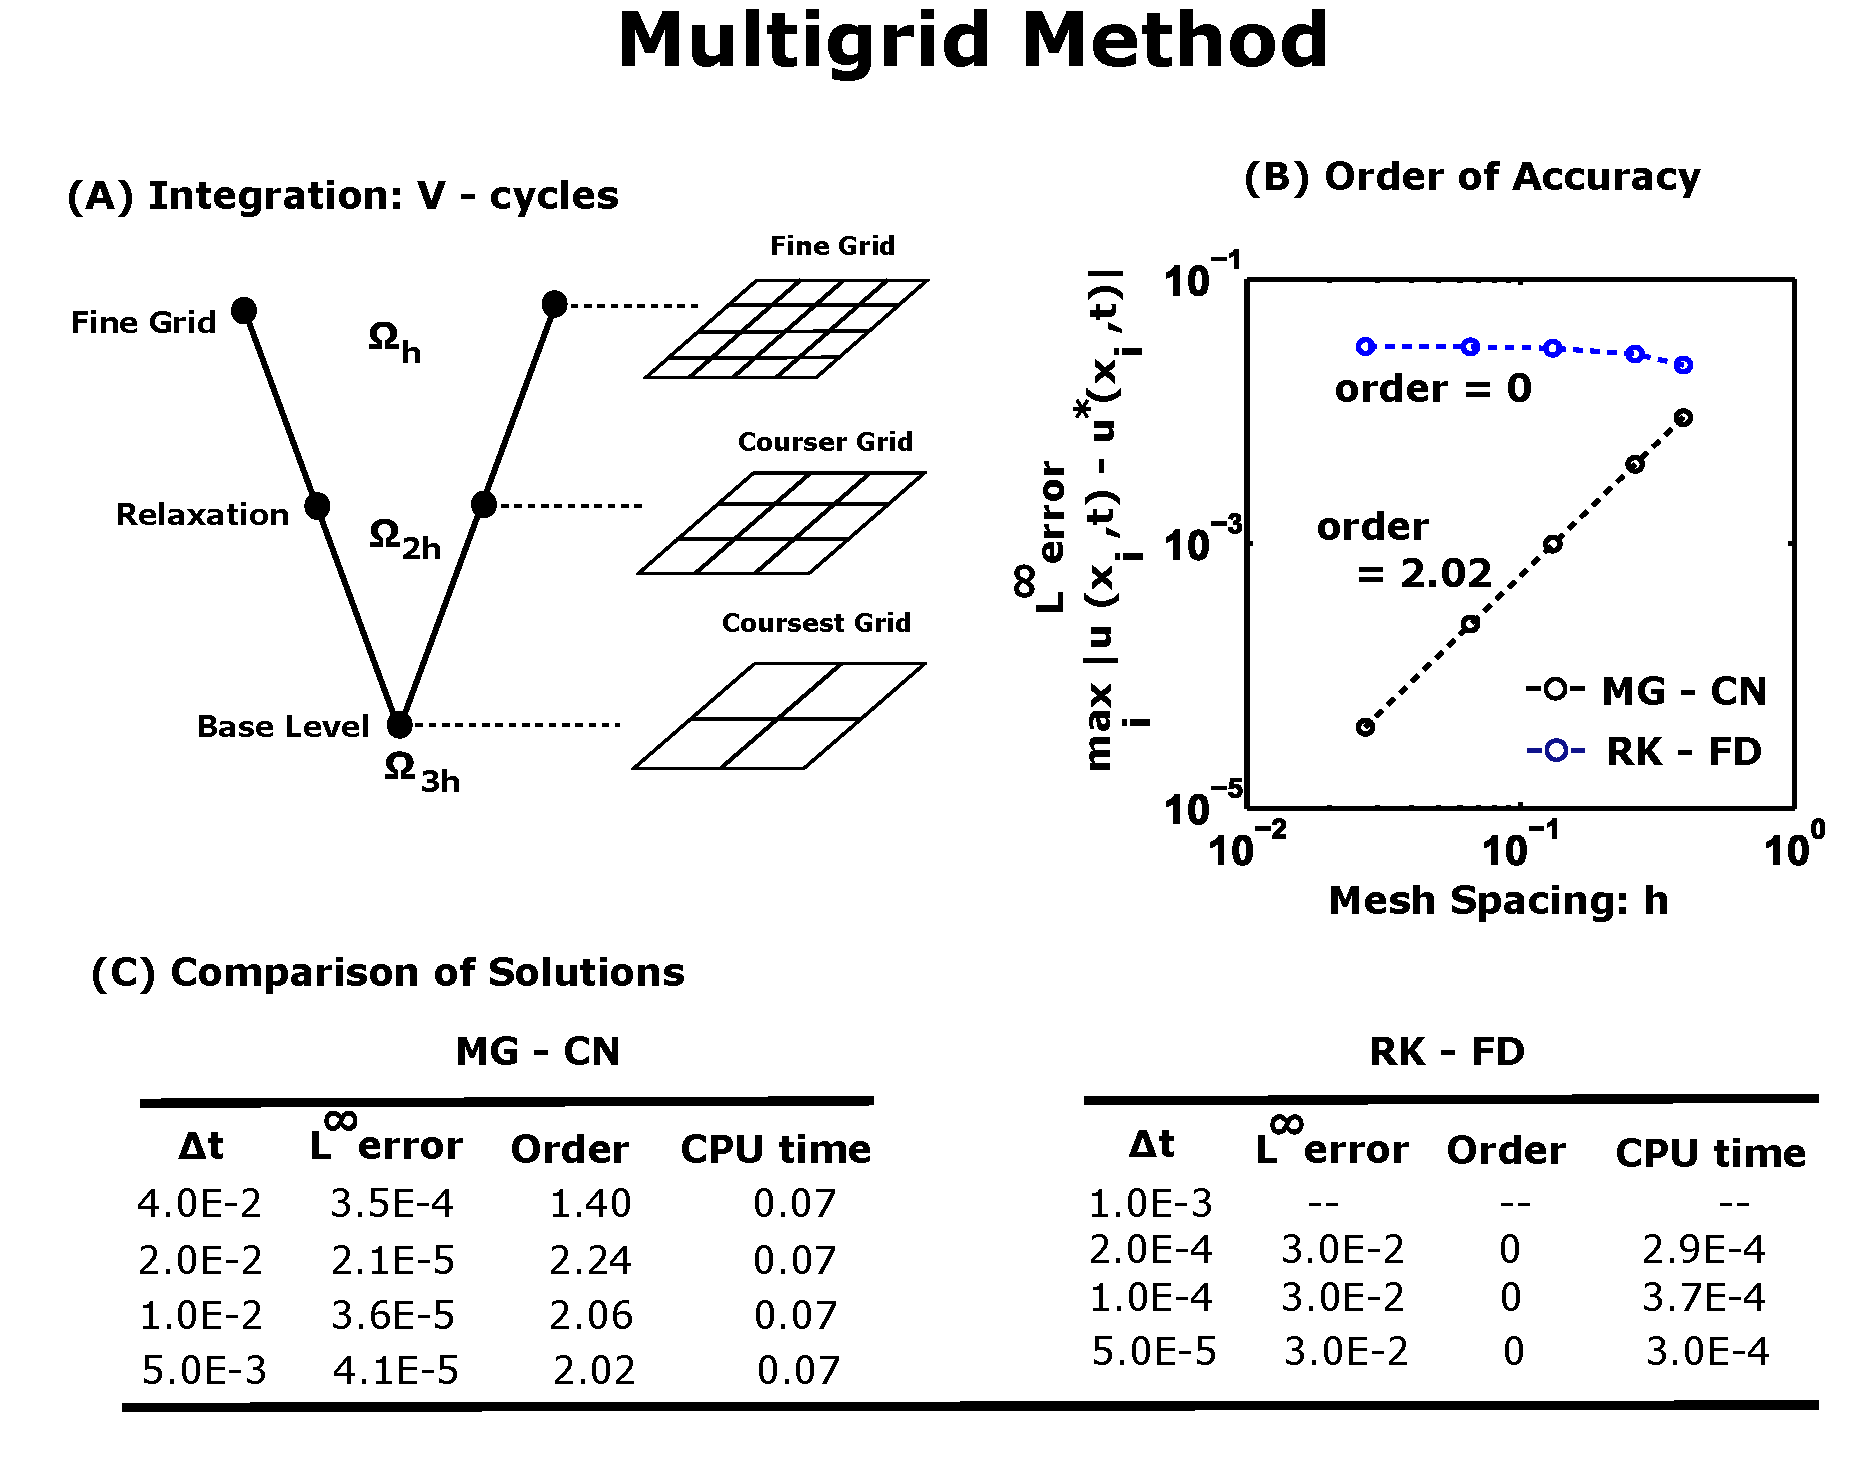
\includegraphics[width=0.6\textwidth]{Multigrid_1D_Results.pdf}
\caption{1-D multigrid V-cycle results from the notes (not used in the main text).}
\label{fig:S_multigrid}
\end{figure}

\paragraph{Population-level agent-based model.} The bacterium--phage life-cycle model (Fig.~\ref{fig:S_abm}) tracks infection, latent period, burst and lysis across a population. This sits one level above the single-cell question studied here. The encounter and binding rates computed in this work are the inputs such a model needs, so it is a natural follow-up, but it is not part of this manuscript.

\begin{figure}[!ht]
\centering
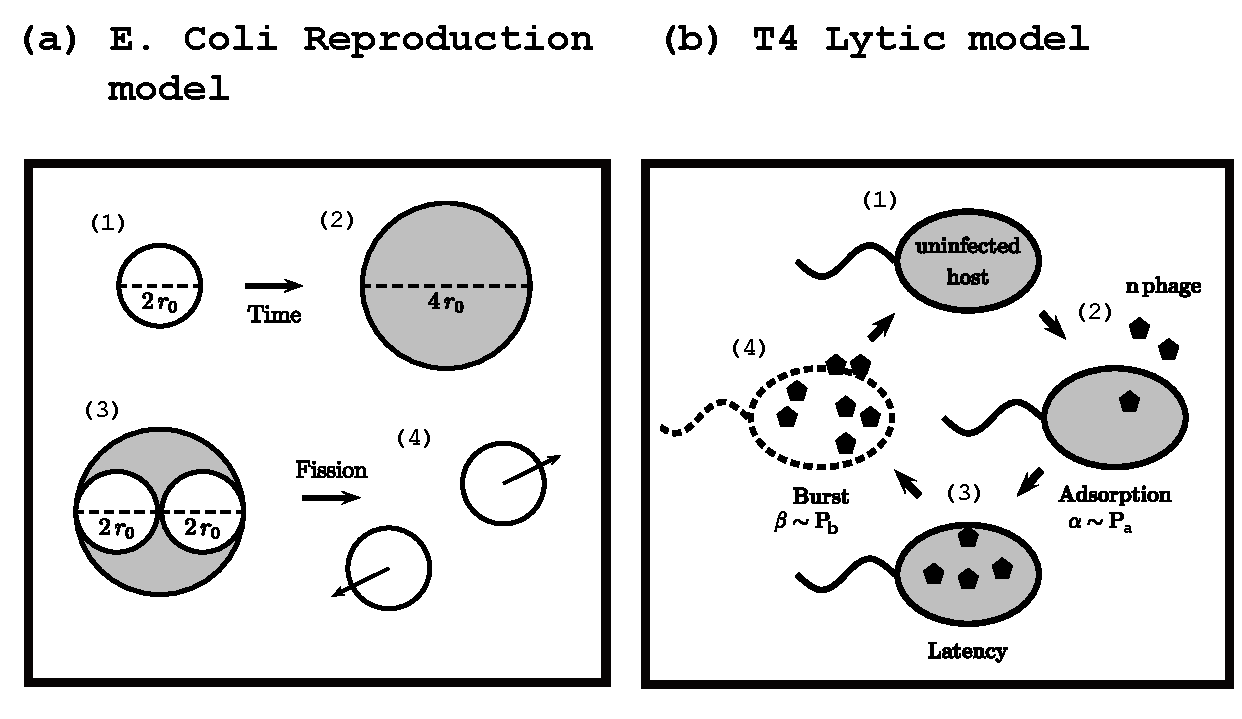
\includegraphics[width=0.45\textwidth]{bac_phage_life.pdf}\hfill
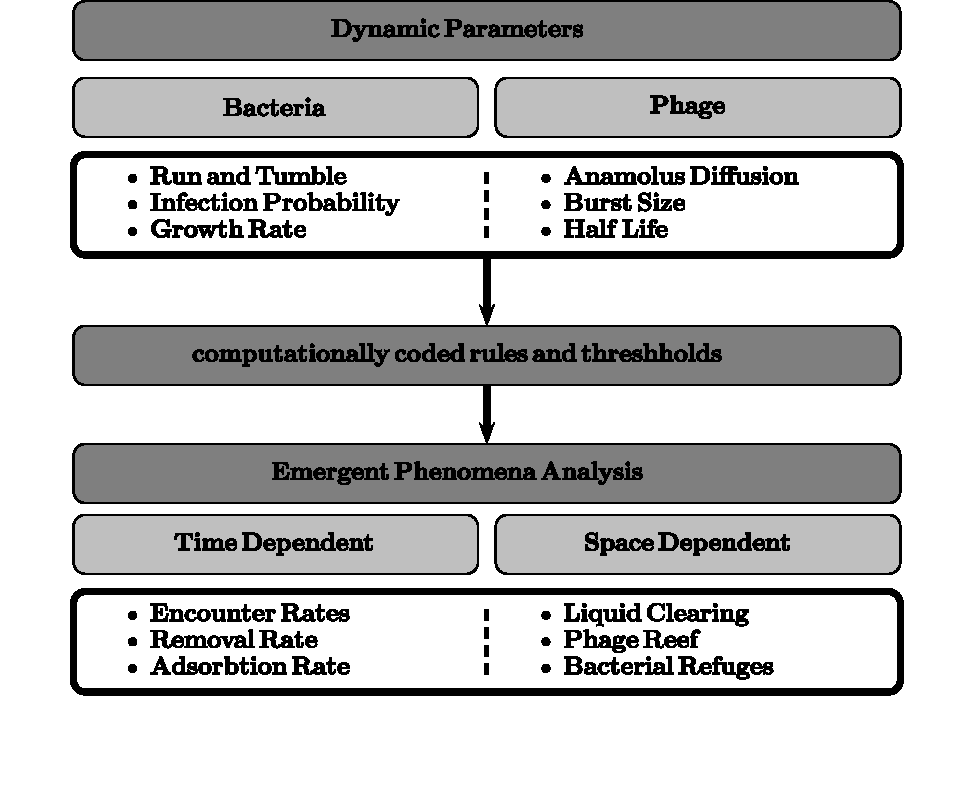
\includegraphics[width=0.45\textwidth]{ABM2.pdf}
\caption{Population-level agent-based model from the notes: life cycle (left) and ABM schematic (right). Out of scope here.}
\label{fig:S_abm}
\end{figure}

\paragraph{Mucus subdiffusion and viscosity.} Subdiffusive phage and the viscosity dependence of swimming speed in mucus were the subject of earlier work\cite{barr2015subdiffusive,joiner2019impact}. The CTRW option (S4) is retained in the code, but all results here use normal diffusion in buffer.

\paragraph{LBM validation (placeholder).} \todo{Add Couette and Poiseuille benchmarks for the D3Q19 solver (velocity profile error versus $\tau$ and resolution), and a comparison of the far-field TIGER flow with a force-dipole (pusher) fit\cite{lauga2016bacterial}.}
